\label{implementation}

This chapter explains implementation details of \tbas\ running on \thismachine.

\section{Keycodes}

\index{keycodes}This is a table of keycodes recognised by the LibGDX, a framework that \thismachine\ runs on.

\begin{longtable}{*{2}{m{\textwidth}}}\hline
\endfirsthead
\endhead

\endfoot
\hline
\endlastfoot
\centering
\begin{tabulary}{\textwidth}{rl}
Key & Code \\
\hline
\ttfamily{1} & 8 \\
\ttfamily{2} & 9 \\
\ttfamily{3} & 10 \\
\ttfamily{4} & 11 \\
\ttfamily{5} & 12 \\
\ttfamily{6} & 13 \\
\ttfamily{7} & 14 \\
\ttfamily{8} & 15 \\
\ttfamily{9} & 16 \\
\ttfamily{0} & 17 \\
$\hookleftarrow$ & 66 \\
\condensedfont{BkSp} & 67 \\
\condensedfont{Tab} & 61 \\
\ttfamily{`} & 68 \\
\ttfamily{'} & 75 \\
\ttfamily{;} & 43 \\
\ttfamily{,} & 55 \\
\ttfamily{.} & 56 \\
\ttfamily{/} & 76 \\
\ttfamily{[}\hspace*{0.083em} & 71 \\
\ttfamily{]}\hspace*{-0.083em} & 72 \\
\ttfamily{-} & 69 \\
\end{tabulary}
\begin{tabulary}{\textwidth}{rl}
Key & Code \\
\hline
\ttfamily{+} & 70 \\
\ttfamily{A} & 29 \\
\ttfamily{B} & 30 \\
\ttfamily{C} & 31 \\
\ttfamily{D} & 32\\
\ttfamily{E} & 33 \\
\ttfamily{F} & 34 \\
\ttfamily{G} & 35 \\
\ttfamily{H} & 36 \\
\ttfamily{I} & 37 \\
\ttfamily{J} & 38 \\
\ttfamily{K} & 39 \\
\ttfamily{L} & 40 \\
\ttfamily{M} & 41 \\
\ttfamily{N} & 42 \\
\ttfamily{O} & 43 \\
\ttfamily{P} & 44 \\
\ttfamily{Q} & 45 \\
\ttfamily{R} & 46 \\
\ttfamily{S} & 47 \\
\ttfamily{T} & 48 \\
\ttfamily{U} & 49 \\
\end{tabulary}
\begin{tabulary}{\textwidth}{rl}
Key & Code \\
\hline
\ttfamily{V} & 50 \\
\ttfamily{W} & 51 \\
\ttfamily{X} & 52 \\
\ttfamily{Y} & 53 \\
\ttfamily{Z} & 54 \\
\condensedfont{LCtrl} & 57 \\
\condensedfont{RCtrl} & 58 \\
\condensedfont{LShift} & 59 \\
\condensedfont{RShift} & 60 \\
\condensedfont{LAlt} & 129 \\
\condensedfont{RAlt} & 130 \\
$\uparrow$ & 19 \\
$\downarrow$ & 20 \\
$\leftarrow$ & 21 \\
$\rightarrow$ & 22 \\
\condensedfont{Ins} & 133 \\
\condensedfont{Del} & 112 \\
\condensedfont{PgUp} & 92 \\
\condensedfont{PgDn} & 93 \\
\condensedfont{Home} & 3 \\
\condensedfont{End} & 132 \\
F1 & 244 \\
\end{tabulary}
\begin{tabulary}{\textwidth}{rl}
Key & Code \\
\hline
F2 & 245 \\
F3 & 246 \\
F4 & 247 \\
F5 & 248 \\
F6 & 249 \\
F7 & 250 \\
F8 & 251 \\
F9 & 252 \\
F10 & 253 \\
F11 & 254 \\
\condensedfont{Num} \ttfamily{0} & 144 \\
\condensedfont{Num} \ttfamily{1} & 145 \\
\condensedfont{Num} \ttfamily{2} & 146 \\
\condensedfont{Num} \ttfamily{3} & 147 \\
\condensedfont{Num} \ttfamily{4} & 148 \\
\condensedfont{Num} \ttfamily{5} & 149 \\
\condensedfont{Num} \ttfamily{6} & 150 \\
\condensedfont{Num} \ttfamily{7} & 151 \\
\condensedfont{Num} \ttfamily{8} & 152 \\
\condensedfont{Num} \ttfamily{9} & 153 \\
\condensedfont{NumLk} & 78 \\
\ttfamily{*} & 17 \\
\end{tabulary}
\end{longtable}

Keys not listed on the table may not be available depending on the system, for example, F12 may not be recognised.

\section{Code Page}
\label{codepage}

\index{code page}By default \thismachine\ uses slightly modified version of CP-437, this is a character map of it:

{\centering
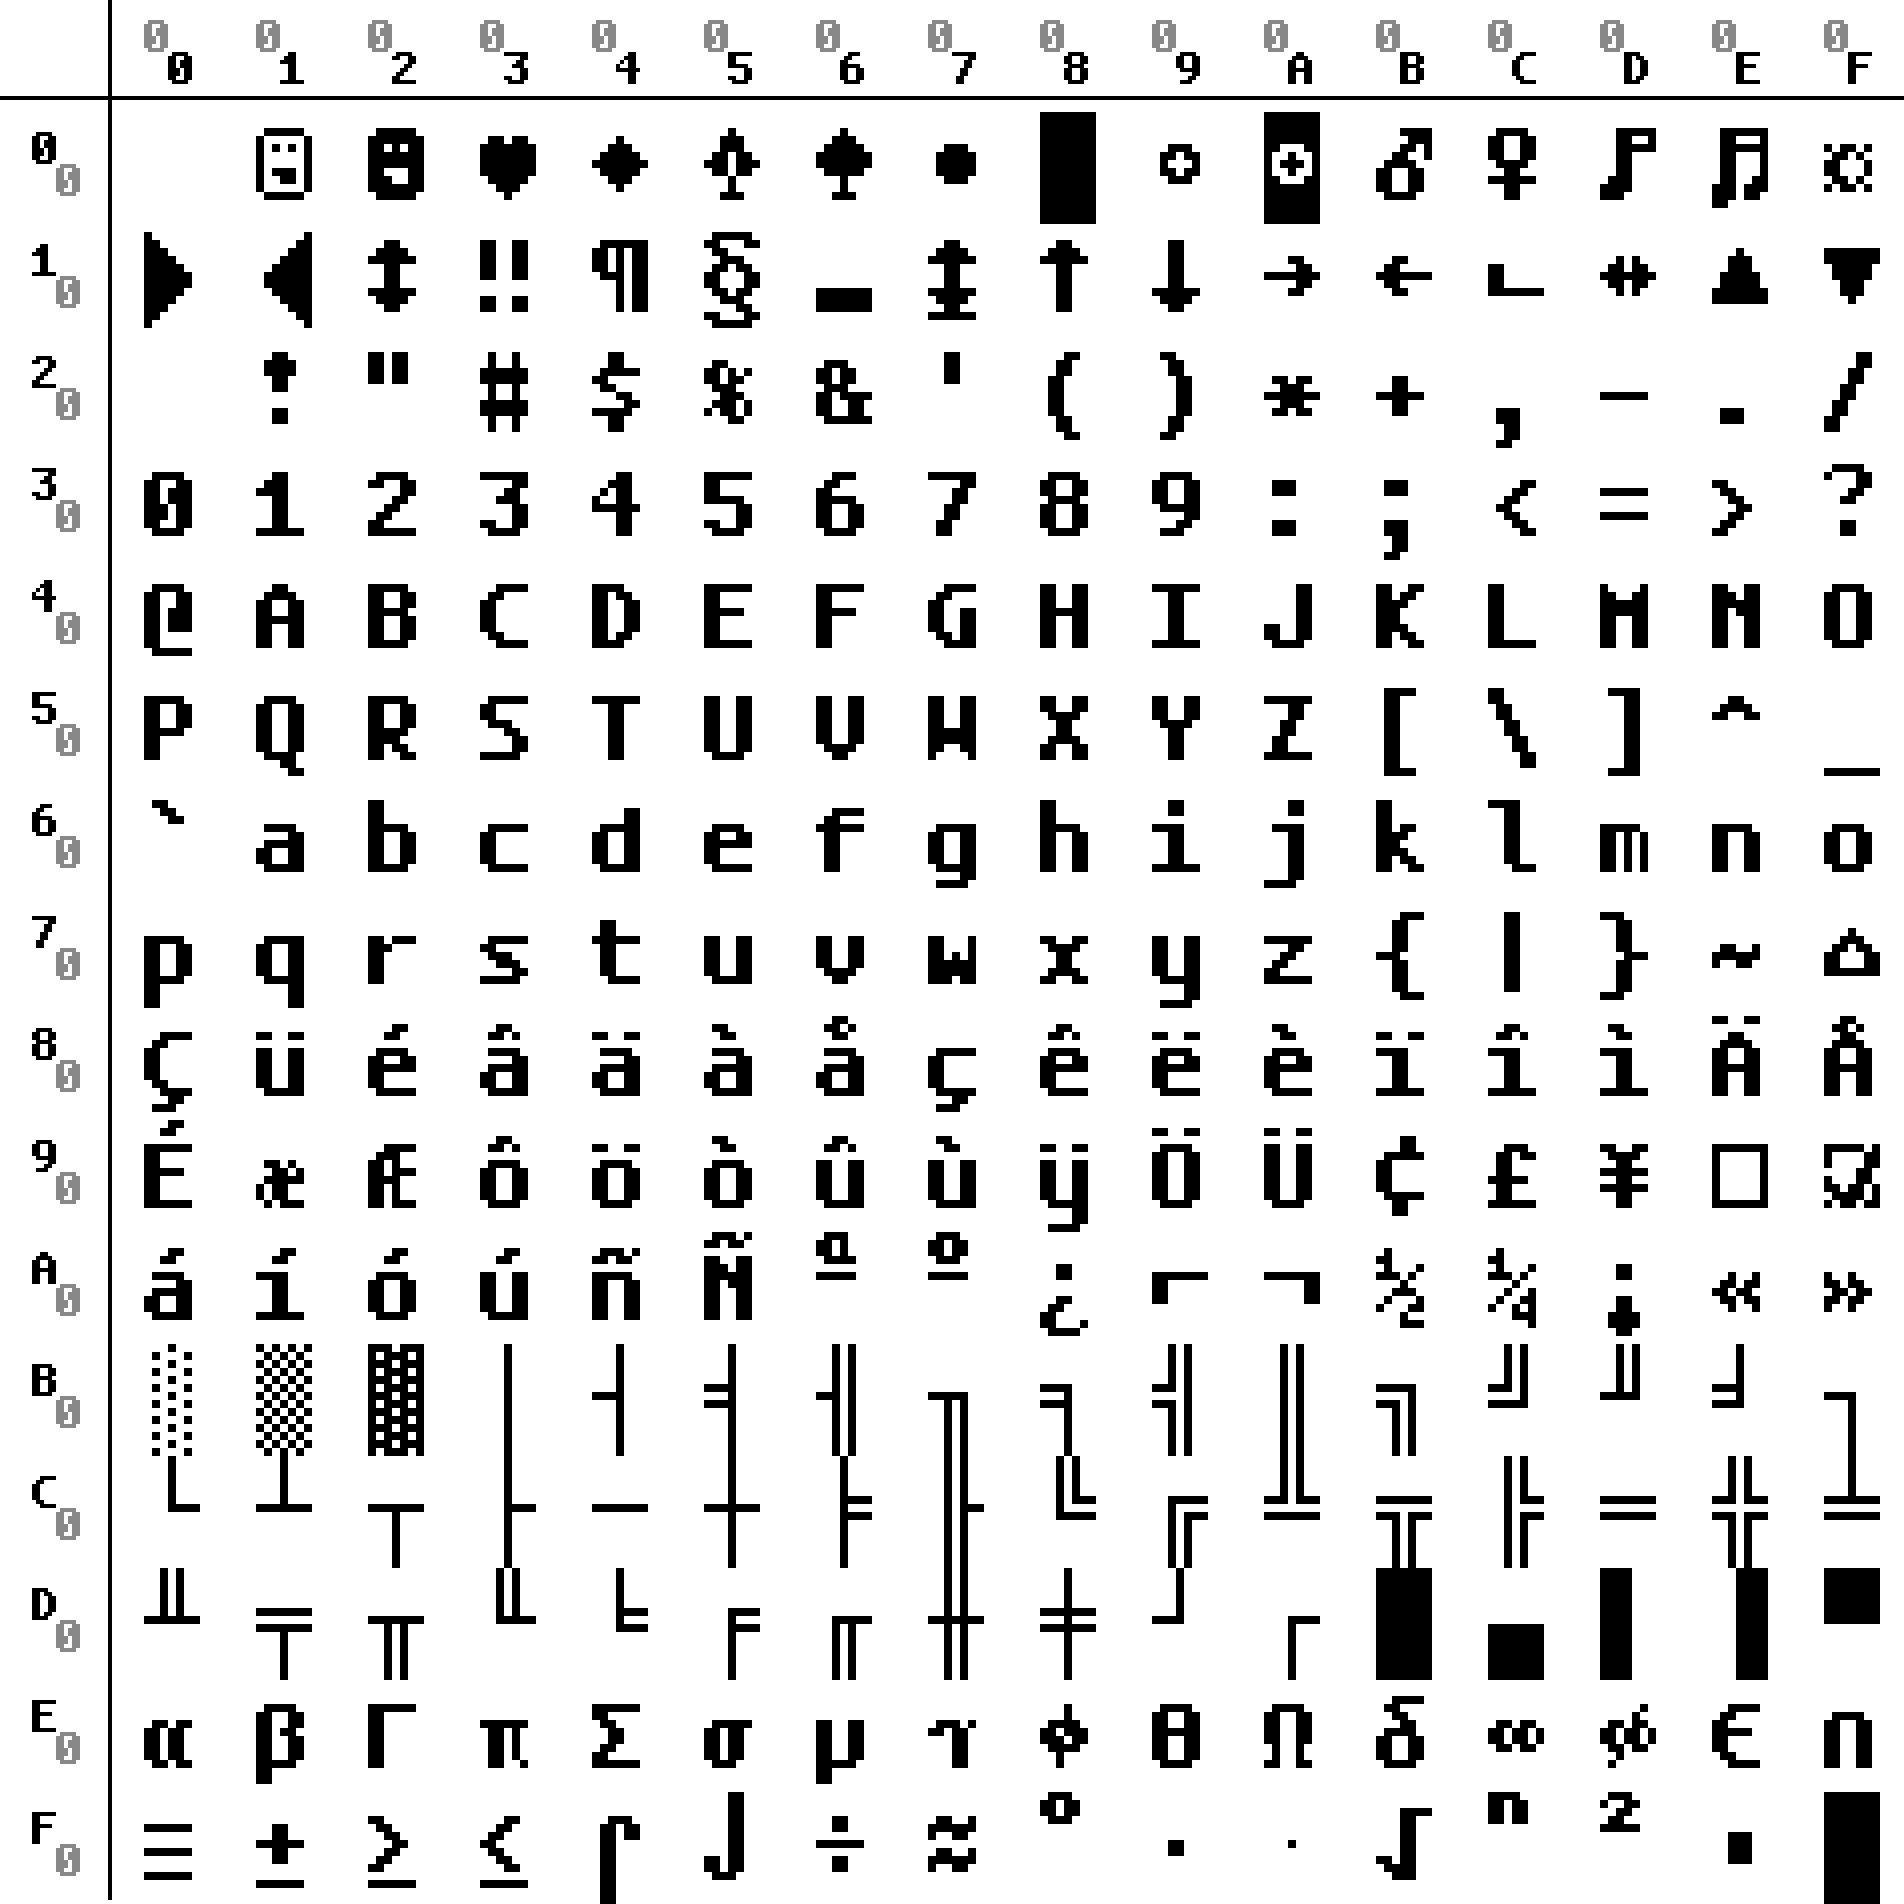
\includegraphics[width=\linewidth]{tsvmcp.png}
\captionof{figure}{\thismachine\ Character Map}
\label{fig:codepage}
}
\newpage

\section{Colour Palette}
\label{colourpalette}

\index{colour palette}By default the reference graphics adapter of the \thismachine\ uses following colour palette:

{\centering
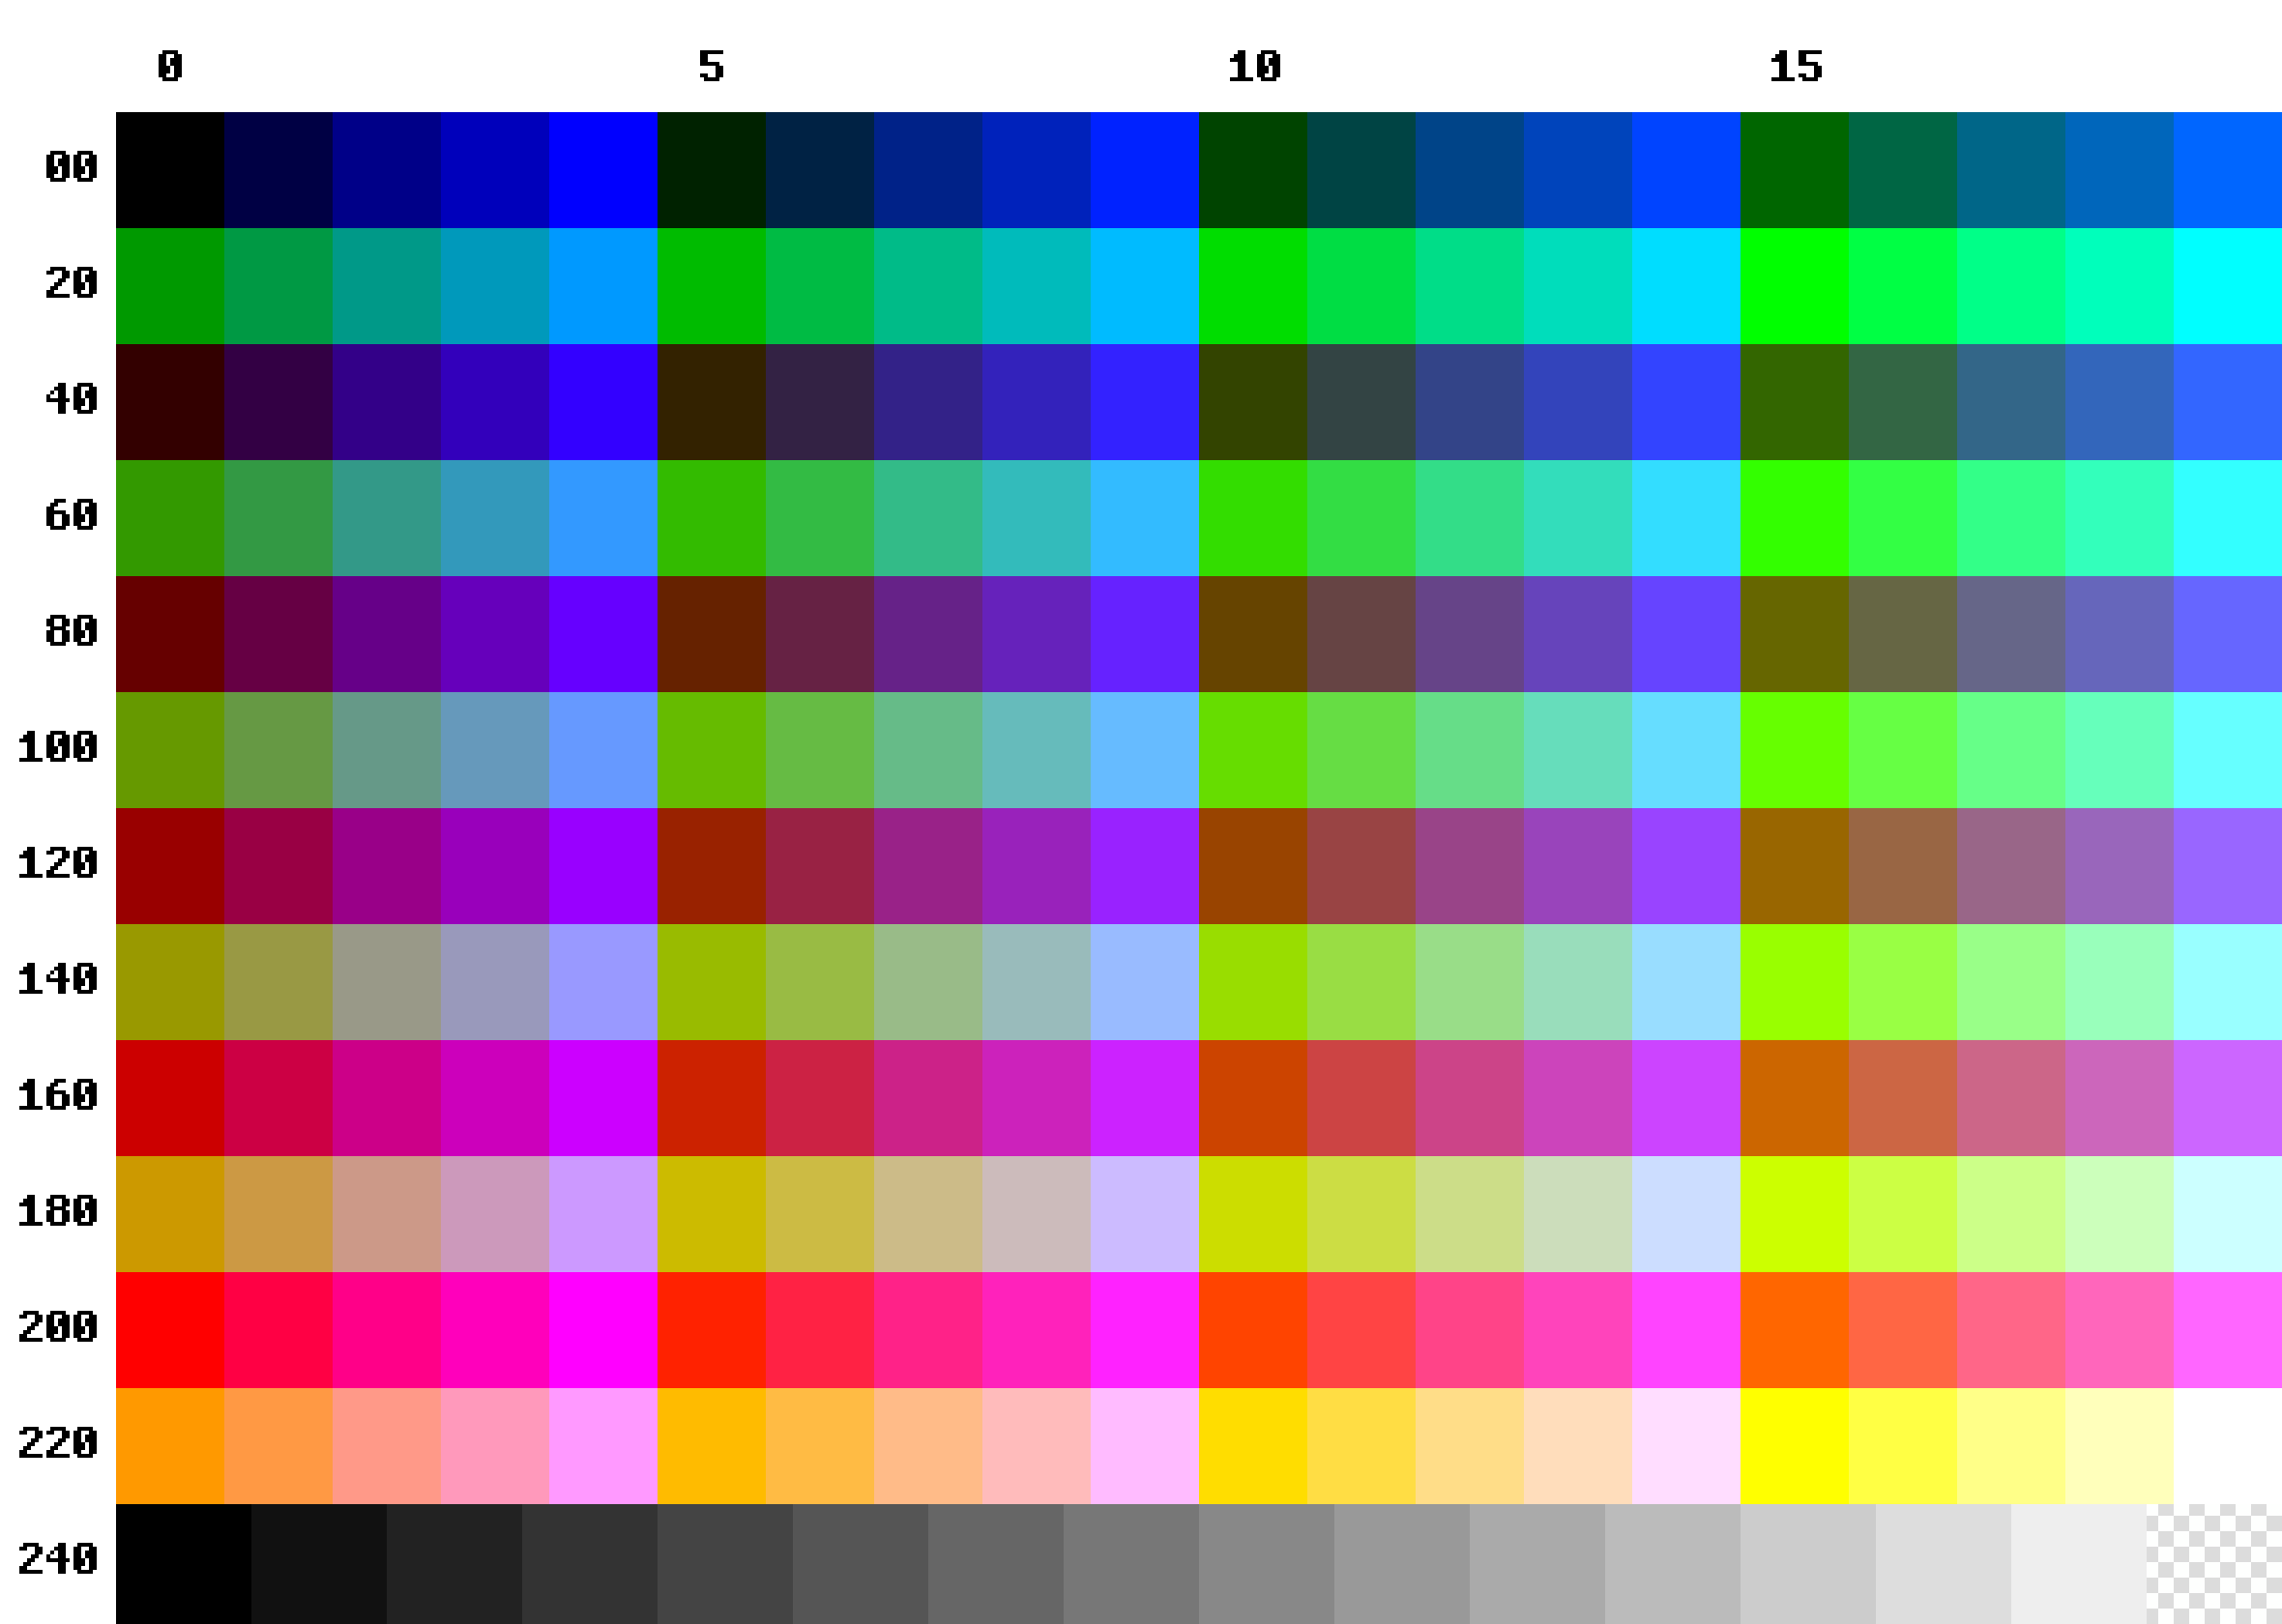
\includegraphics[width=\linewidth]{tsvmpal.png}
\captionof{figure}{\thismachine\ Colour Palette}
\label{fig:codepage}
}
